\chapter{弱場、引力波與作用量原理}

廣義相對論的精確方程是非線性的；在解決任何物理問題之前，光是寫出分量形式就可能繁複得令人難以招架。作為本課程的最後一講，適合先把原理和繁複的計算分開。我們將探討引力場微弱時愛因斯坦方程會變成什麼樣子，辨認這個近似中包含的波，最後再看看完整的場方程如何納入一個極為簡潔的作用量原理。

這場討論圍繞三個問題展開：弱引力場是什麼意思？為什麼精確理論是非線性的，弱場理論卻是線性的？又有哪些物理效應能區分引力波和單純的座標抖動？

\section{平衡幾何的微小擾動}

「弱」是一種近似方案。若無量綱擾動的量級為\(\epsilon\ll1\)，其平方的量級便是\(\epsilon^2\)；一致地進行一階計算時，後者會被捨去。熟悉的例子是力學系統在平衡位置附近作小振動。它的精確方程可能是非線性的，但振動幅度足夠小時，便服從線性方程。

對引力而言，平衡背景取為真空中的平直時空。從愛因斯坦真空方程出發，
\begin{equation}
 R_{\mu\nu}-\frac12 g_{\mu\nu}R=0.
 \label{eq:l10-vacuum-einstein}
\end{equation}
在四維時空中取跡，得到
\begin{equation}
 g^{\mu\nu}
 \left(R_{\mu\nu}-\frac12 g_{\mu\nu}R\right)
 =R-2R=-R=0,
\end{equation}
因此，真空方程等價於
\begin{equation}
 R_{\mu\nu}=0.
 \label{eq:l10-ricci-flat}
\end{equation}

\begin{figure}[htbp]
\centering
\includegraphics[width=0.68\textwidth]{lecture_10_figure_02.png}
\caption{在弱場論證開頭單獨列出的真空方程 \(R_{\mu\nu}=0\)。}
\lectureframe{00:03:11}
\end{figure}

這裡的「平衡」是指沒有源、且不隨時間變化的解。平直時空是最簡單的此類解。有一點限定至關重要：平直並不表示度規分量在每個座標系中都等於某個特定矩陣，而是表示可以選取慣性座標，使得
\begin{equation}
 g_{\mu\nu}=\eta_{\mu\nu}.
\end{equation}
幾何與描述幾何所用座標之間的區別，很快就會成為核心的微妙之處。

現在設想一個劇烈的源，例如緻密雙星。它的近場可能很強，但離源越遠，擾動越向外傳播，也越微弱。在適當的座標系中，度規便可寫成
\begin{equation}
 g_{\mu\nu}(x)=\eta_{\mu\nu}+h_{\mu\nu}(x),
 \qquad |h_{\mu\nu}|\ll1.
 \label{eq:weak-split}
\end{equation}
擾動\(h_{\mu\nu}\)可以依賴全部四個時空座標。所謂微弱，表示高於一階的項都會被忽略。

\section{一階近似下留下的項}

完整的里奇張量在此階段過於冗長，無助於理解；掌握它的結構就足夠了。克里斯托費爾符號包含逆度規和度規的一階導數，而曲率則包含克里斯托費爾符號的導數，以及兩個克里斯托費爾符號的乘積：
\begin{equation}
 \Gamma\sim\frac12 g^{-1}\partial g,
 \qquad
 R\sim\partial\Gamma+\Gamma\Gamma.
 \label{eq:curvature-skeleton}
\end{equation}

\begin{figure}[htbp]
\centering
\includegraphics[width=0.84\textwidth]{lecture_10_figure_03.png}
\caption{弱場拆分與示意性的構造 \(R\sim\partial\Gamma+\Gamma\Gamma\)。這種記法顯示了\(h\)的各階，而不必展開每個指標。}
\lectureframe{00:10:17}
\end{figure}

由
\(g^{\mu\alpha}g_{\alpha\nu}=\delta^\mu{}_\nu\)可求得逆度規。保留到一階，
\begin{equation}
 g^{\mu\nu}=\eta^{\mu\nu}-h^{\mu\nu}+O(h^2),
 \label{eq:inverse-weak}
\end{equation}
其中\(h\)的指標以背景度規升降。在慣性座標中，背景度規是常數，
\begin{equation}
 \partial_\alpha\eta_{\mu\nu}=0,
\end{equation}
因此
\begin{equation}
 \partial_\alpha g_{\mu\nu}
 =\partial_\alpha h_{\mu\nu}.
\end{equation}
於是，
\begin{equation}
\begin{aligned}
 \Gamma&=O(\partial h),\\
 R_{\mu\nu}
 &=O(\partial\partial h)+O\bigl((\partial h)^2\bigr)\\
 &\quad+O(h\,\partial\partial h).
\end{aligned}
 \label{eq:ricci-orders}
\end{equation}

\begin{figure}[htbp]
\centering
\includegraphics[width=0.84\textwidth]{lecture_10_figure_04.png}
\caption{黑板上對逆度規的展開，以及\(\partial\eta=0\)這一觀察。領先階只留下\(h_{\mu\nu}\)的導數。}
\lectureframe{00:11:55}
\end{figure}

方程~\eqref{eq:ricci-orders}中的最後兩項是擾動的二階項，因此略去。真空方程於是成為涉及\(h_{\mu\nu}\)二階導數的線性方程。這就是線性化的全部意思；它並不是說愛因斯坦的精確理論是線性的。

\begin{classroomqa}
\audiencequestion{曲率張量有四個指標，里奇張量則有兩個。如果兩個導數已經帶有指標，而\(h_{\mu\nu}\)又帶有另外兩個指標，指標數目怎麼能對得上？}
\lecturerresponse{里奇張量是將曲率張量的一對指標縮並而得。縮並所用的度規留下兩個自由指標，正好就是\(R_{\mu\nu}\)所帶的那一對。符號形式\(\partial\partial h\)省略了這些縮並；它只是在計算階數，並不是完整的指標公式。
\lecturetimestamp{00:18:45--00:19:53}}
\end{classroomqa}

\begin{classroomqa}
\audiencequestion{用逆度規縮並時，會不會引入像\(h\,\partial^2h\)這樣的項？如果會，為什麼可以忽略？}
\lecturerresponse{會。將\(g^{-1}\)換成
\(\eta^{-1}-h+\cdots\)會同時得到線性項
\(\eta^{-1}\partial^2h\)，以及含有另一個\(h\)的修正項。後者是二階項。同樣的規則也會略去
\(h\,\partial h\)、\(h\,\partial^2h\)和
\((\partial h)^2\)。只保留擾動的一次項，正是這裡採用的近似。
\lecturetimestamp{00:19:55--00:21:14}}
\end{classroomqa}

\section{為什麼方程看起來像波動方程}

含有二階導數的場方程，自然會讓人想到波的傳播。對於沿\(z\)軸傳播的純量場，典型的波動方程是
\begin{equation}
 \left(\partial_t^2-\partial_z^2\right)\phi=0,
\end{equation}
其解包括任意向右和向左傳播的波形，
\begin{equation}
 \phi(z,t)=f(z-t)+g(z+t).
\end{equation}
在三維空間中，同一方程寫作
\begin{equation}
 \left(\partial_t^2-\nabla^2\right)\phi=0.
\end{equation}
由於方程是線性的，解可以疊加：兩個解相加仍然是解。

引力不是純量場。擾動有張量分量，而方程\(R_{\mu\nu}=0\)乍看之下似乎提供了許多分量方程。但這些方程並非全都獨立；有些是約束，有些則反映座標自由度。這和麥克斯威理論類似：一組場方程最後只留下物理的橫向波。

施加適當的座標條件後，輻射分量便服從一般的波動方程，
\begin{equation}
 \Box h_{\mu\nu}=0,
 \qquad
 \Box=\eta^{\alpha\beta}\partial_\alpha\partial_\beta.
 \label{eq:linear-wave}
\end{equation}
\(\Box\)中的確切正負號取決於度規號差慣例，但方程的物理內容不受影響。擾動沿光錐傳播。

\section{座標抖動不是引力波}

在把線性化方程的每個解都視為物理波之前，我們得先回到座標上的注意事項。平直空間也能用彎曲的座標線來描述。如此一來，即使曲率仍為零，度規分量也會不同於笛卡兒座標中的值。

黑板本身就能說明這一點。在平坦的黑板表面畫上直的笛卡兒座標線，並寫下
\begin{equation}
 ds^2=\delta_{mn}\,dx'^m dx'^n.
\end{equation}
接著用略微彎曲的座標重新標記相同的點，
\begin{equation}
 x'^m=x^m+f^m(x).
 \label{eq:small-coordinate-change}
\end{equation}
微分便變成
\begin{equation}
 dx'^m=dx^m+\partial_n f^m\,dx^n.
\end{equation}
代入線元素，並只保留\(f\)的一階項，得到
\begin{align}
 ds^2
 &=\delta_{mn}dx^m dx^n\\
 &\quad+\left(\partial_m f_n+\partial_n f_m\right)dx^m dx^n
 +O(f^2).
\end{align}
因此，形如
\begin{equation}
 h_{mn}=\partial_m f_n+\partial_n f_m
 \label{eq:pure-gauge}
\end{equation}
的表觀擾動，完全可能沒有帶來任何新的幾何；它只是以彎曲座標表示的平直空間。

\begin{figure}[htbp]
\centering
\includegraphics[width=0.84\textwidth]{lecture_10_figure_05.png}
\caption{黑板上的座標抖動計算。微小的座標重標記會引出一個看似微小的\(h_{mn}\)，但黑板仍然是平直的。}
\lectureframe{00:27:54}
\end{figure}

方程~\eqref{eq:pure-gauge}是座標自由度（亦即規範自由度）的線性化形式。要消除這些虛假的擾動，還需要附加條件。這裡不推導詳細的規範代數；要點在於它的作用：去除描述方式的改變，同時保留曲率的改變。計入座標自由度和約束方程後，物理內容只剩下兩種獨立的波偏振。

\begin{figure}[htbp]
\centering
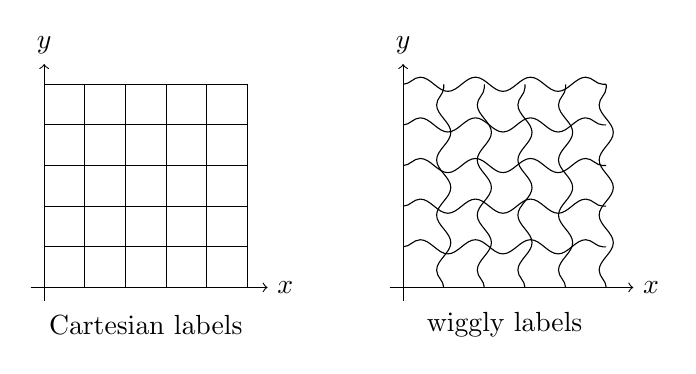
\begin{tikzpicture}[scale=0.86]
\begin{scope}
\draw[->] (-0.2,0) -- (3.3,0) node[right] {$x$};
\draw[->] (0,-0.2) -- (0,3.3) node[above] {$y$};
\foreach \u in {0.6,1.2,1.8,2.4,3.0}{
  \draw (\u,0) -- (\u,3.0);
  \draw (0,\u) -- (3.0,\u);
}
\node at (1.5,-0.55) {Cartesian labels};
\end{scope}
\begin{scope}[xshift=5.3cm]
\draw[->] (-0.2,0) -- (3.4,0) node[right] {$x$};
\draw[->] (0,-0.2) -- (0,3.3) node[above] {$y$};
\foreach \u in {0.6,1.2,1.8,2.4,3.0}{
  \draw[decorate,decoration={snake,amplitude=0.09cm,segment length=0.7cm}]
    (\u,0) -- (\u,3.0);
  \draw[decorate,decoration={snake,amplitude=0.09cm,segment length=0.7cm}]
    (0,\u) -- (3.0,\u);
}
\node at (1.5,-0.55) {wiggly labels};
\end{scope}
\end{tikzpicture}
\caption{幾何保持平直，座標網格則有所改變。單憑度規分量，無法判斷某個擾動是否具有物理意義。}
\end{figure}

\section{沿 z 軸傳播的波}

考慮一列沿\(z\)正方向傳播的平面波。它的相位可寫為
\begin{equation}
 k(z-t),
\end{equation}
因此，一個代表性的分量具有以下形式：
\begin{equation}
 h_{\mu\nu}(z,t)
 =h_{\mu\nu}^{(0)}\sin k(z-t).
 \label{eq:plane-wave}
\end{equation}
等相位面滿足\(z-t=\text{constant}\)，所以傳播速度就是光速。

在橫向無跡表述中，帶有時間指標或\(z\)指標的分量都為零：
\begin{equation}
 h_{0\mu}=0,
 \qquad
 h_{z\mu}=0.
 \label{eq:tt-transverse}
\end{equation}
只留下\(x\)-\(y\)區塊。這個區塊是對稱且無跡的：
\begin{equation}
 h_{xy}=h_{yx},
 \qquad
 h_{xx}+h_{yy}=0.
 \label{eq:tt-trace}
\end{equation}

\begin{figure}[htbp]
\centering
\includegraphics[width=0.84\textwidth]{lecture_10_figure_06.png}
\caption{沿\(z\)傳播的波，可表示為一疊橫向平面。留下的\(x\)-\(y\)振幅滿足\(h_{xx}+h_{yy}=0\)。}
\lectureframe{00:43:36}
\end{figure}

因此只有兩種獨立的模式。對於\(i,j\in\{x,y\}\)，可將它們寫成
\begin{equation}
 h^{\mathrm{TT}}_{ij}(z,t)
 =
 \begin{pmatrix}
 h_+ & h_\times\\
 h_\times & -h_+
 \end{pmatrix}
 \sin k(z-t).
 \label{eq:polarization-matrix}
\end{equation}
對角模式稱為加偏振，非對角模式稱為叉偏振。將橫向座標軸旋轉\(45^\circ\)，一種模式便會轉成另一種；任意的線偏振波都可以表示為兩者的疊加。在這套理論中，沒有其他獨立偏振。

\begin{figure}[htbp]
\centering
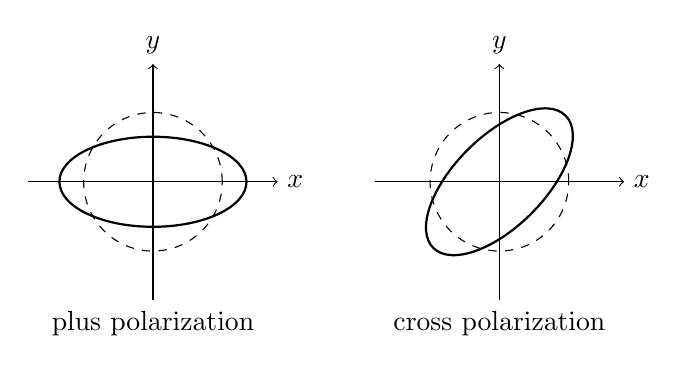
\begin{tikzpicture}[scale=0.88]
\begin{scope}
\draw[->] (-1.8,0) -- (1.8,0) node[right] {$x$};
\draw[->] (0,-1.7) -- (0,1.7) node[above] {$y$};
\draw[dashed] (0,0) circle (1.0);
\draw[thick] (0,0) ellipse (1.35 and 0.65);
\node at (0,-2.05) {plus polarization};
\end{scope}
\begin{scope}[xshift=5.0cm]
\draw[->] (-1.8,0) -- (1.8,0) node[right] {$x$};
\draw[->] (0,-1.7) -- (0,1.7) node[above] {$y$};
\draw[dashed] (0,0) circle (1.0);
\draw[thick,rotate=45] (0,0) ellipse (1.35 and 0.65);
\node at (0,-2.05) {cross polarization};
\end{scope}
\end{tikzpicture}
\caption{在半個週期內，一個橫向方向被拉長，與其垂直的方向則被壓縮；再過半個週期，形變便反轉。}
\end{figure}

\section{從度規分量到物理應變}

固定\(z\)和\(t\)，觀察橫向平面。對純加偏振波，
\begin{equation}
 ds_\perp^2
 =(1+h_{xx})\,dx^2+(1-h_{xx})\,dy^2.
 \label{eq:transverse-distance}
\end{equation}
當\(h_{xx}>0\)時，\(x\)方向上的固定座標間隔，其固有長度會稍微增加；相應的\(y\)方向間隔，其固有長度則會稍微減少。半個週期後，\(h_{xx}\)改變符號，兩個方向的變化便互換。一個正方形會先在水平方向拉長、在垂直方向壓縮，接著在水平方向壓縮、在垂直方向拉長。叉偏振也會以相同方式交替形變，只是方向沿著旋轉\(45^\circ\)的座標軸。

一條初始長度為\(L\)的臂，其長度變化在一階近似下為
\begin{equation}
 \frac{\Delta L}{L}\simeq\frac12 h_{ij}n^i n^j,
 \label{eq:fractional-strain}
\end{equation}
其中\(\mathbf n\)是沿著臂的單位向量。這個公式將度規擾動轉換為探測器量得的無量綱應變。

\begin{classroomqa}
\audiencequestion{米尺靠電磁力維持形狀，不會隨座標改變而簡單地改變靜止長度。圖中是否應改用彼此分離的自由檢驗質量？}
\lecturerresponse{這個區別很重要。真實的桿具有彈性，所以潮汐場會在桿內產生應力；鋼桿和木桿通常會有不同的反應。自由懸掛的檢驗質量不會有這種特定的彈性反應，因此能更直接地呈現相對加速度。無論採用哪一種方式，經過的波都不只是重新標記各個位置。隨時間變化的曲率會產生實際的物理效應。
\lecturetimestamp{00:47:23--00:48:48}}
\end{classroomqa}

精確的局域描述是測地線偏離。對於彼此相隔\(\xi^i\)的鄰近自由落體粒子，
\begin{equation}
 \frac{d^2\xi^i}{dt^2}
 =-R^i{}_{0j0}\,\xi^j.
 \label{eq:geodesic-deviation}
\end{equation}
在弱場的橫向無跡波中，
\begin{equation}
 R_{0i0j}=-\frac12\ddot h^{\mathrm{TT}}_{ij},
 \label{eq:tidal-curvature}
\end{equation}
因此，振盪的度規會產生交替的潮汐加速度。隨時間變化的波之所以不能被當成靜態的尺規選擇而排除，就是因為它具有非零曲率。

\begin{classroomqa}
\audiencequestion{如果區域內所有尺子都受到影響，還能用什麼測量拉伸和壓縮？}
\lecturerresponse{應變計可以記錄材料物體中實際產生的應力。更好的方法是監測自由懸掛質量之間不斷改變的距離。靜態且均勻的尺度改變可以併入測量儀器的設定；但振盪的曲率會驅動可記錄的響應。
\lecturetimestamp{00:51:10--00:52:02}}
\end{classroomqa}

\section{波源與探測器}

電磁波由運動的電荷與電流產生；引力波則由運動的質量與能量分佈產生。能量和動量守恆排除了孤立系統的引力單極與偶極輻射，因此最主要的輻射多極矩是四極矩。緻密雙星恰好提供了所需的變化四極矩：兩個緻密天體互相繞行，並向遠場發射波。

在雙星附近，時空的曲率很強，方程~\eqref{eq:weak-split}的線性展開並不可靠。遠離雙星時，出射波散布到更大的面積，振幅因而減小，線性化描述也就準確起來。對位於波源\(z\)軸方向的觀測者而言，可測得的拉伸發生在橫向的\(x\)-\(y\)平面內。

\begin{classroomqa}
\audiencequestion{圖中的尺子是抽象的座標尺，還是實際的米尺？如果尺子本身長度會變，又怎麼能用它測量這個效應？}
\lecturerresponse{尺子可以是實際物體，但這時材料性質就很重要。曲率會產生潮汐應力；鋼和木材受到這種應力時，形變不必相同。比較兩者的反應，本身就是一種測量。更直接的探測器會以彼此分離的檢驗質量取代桿，測量它們之間的差異運動。
\lecturetimestamp{00:54:00--00:55:19}}
\end{classroomqa}

共振探測器是一種方法。如果機械系統的固有頻率接近入射波的頻率，波便能持續地驅動系統，放大其響應。干涉儀則採用另一種方法：以反射鏡作為檢驗質量，利用雷射干涉比較互相垂直兩臂的有效長度。加偏振波會使一條臂變長、另一條臂變短；干涉儀正是用來偵測這種長度差異訊號。

\begin{classroomqa}
\audiencequestion{這會是引力波探測器的原理嗎？}
\lecturerresponse{是的。堅硬的桿幾乎不會改變長度，但自由懸掛的端點質量可以產生相對加速度。也可以利用共振，讓微弱的週期性驅動產生較大的響應。預期的天體物理應變極其微小，量級約為\(10^{-21}\)；探測器設計的關鍵，便是把這種微小的差異運動轉換成可測量的訊號。
\lecturetimestamp{00:55:20--00:57:10}}
\end{classroomqa}

\begin{classroomqa}
\audiencequestion{LIGO 是這類探測器的例子嗎？}
\lecturerresponse{是。它的基本觀測量來自雷射光在互相垂直的兩臂中，於鏡面之間反射所形成的訊號。引力波會改變兩臂的相對光程，進而改變干涉圖樣。這場講座當時，儀器尚未直接探測到引力波；後來情況已有所改變。\editorialnote{首次直接觀測到的事件 GW150914，記錄於2015年，並於2016年宣布。}
\lecturetimestamp{00:57:16--00:58:05}}
\end{classroomqa}

\begin{classroomqa}
\audiencequestion{波動解所預測的傳播速度是多少？}
\lecturerresponse{光速。相位\(k(z-t)\)在\(z\)方向每前進一個單位，\(t\)方向也前進一個單位；線性化的愛因斯坦方程與電磁波方程具有相同的光錐傳播結構。
\lecturetimestamp{00:58:07--00:58:16}}
\end{classroomqa}

黑洞碰撞和緻密雙星是特別有希望的波源。碰撞附近的引力場高度非線性，釋放出的能量可能有相當大一部分以引力輻射的形式離開。訊號抵達遙遠的探測器時，振幅已微弱到足以用線性波傳播作為極佳的描述。引力輻射因此開啟了一種不必仰賴光訊號的天文觀測途徑。

\section{雙星脈衝星與間接證據}

輻射會攜帶能量。如果雙星發射引力波，軌道能量便會減少，兩個天體會緩慢地向內旋近，軌道週期也會改變。雙星脈衝星提供了足夠精確的時鐘，能測量這種變化。其觀測到的軌道演化，在數值上與廣義相對論預測的能量損失一致。

在這場講座所處的歷史背景下，這是決定性的間接證據：當時尚無探測器記錄到引力波穿越地球，但雙星軌道確實正以引力輻射所預測的速率損失能量。即使尚未直接接收到波，仍可透過波對波源造成的影響觀測到它們。

\begin{classroomqa}
\audiencequestion{最初被研究的雙星脈衝星系統，其頻率或週期是多少？是在毫秒尺度嗎？}
\lecturerresponse{毫秒尺度指的是脈衝星的自轉週期，不是兩顆星的軌道週期。課堂上查核後得知，軌道週期約為\(7.75\)小時。這個區別很重要：引力輻射反映的是雙星的軌道運動，而射電脈衝則提供追蹤軌道變化所需的精確時鐘。
\lecturetimestamp{01:01:27--01:03:28}}
\end{classroomqa}

\begin{classroomqa}
\audiencequestion{數十年的觀測期間，累積的軌道計時變化有多大？}
\lecturerresponse{所引述的累積偏移約為三十秒。瞬時相對變化雖然極小，但經過數十年的精確脈衝計時，累積效應便清楚可見。
\lecturetimestamp{01:03:34--01:03:54}}
\end{classroomqa}

\section{時間依賴性、曲率與線性近似的適用範圍}

\begin{classroomqa}
\audiencequestion{為什麼選擇橫向的\(x\)-\(y\)平面？如果改看由\(x\)和\(t\)所張成的平面，又會如何？}
\lecturerresponse{波本身依賴\(z\)和\(t\)，但「橫向」指的是垂直於波的空間傳播方向的空間方向。對於沿\(z\)方向傳播的波，可以把物理度規振幅選在\(x\)-\(y\)區塊中。其他表觀分量則不存在，或可透過座標選擇移除。
\lecturetimestamp{01:02:22--01:03:17}}
\end{classroomqa}

\begin{classroomqa}
\audiencequestion{是時間本身在振盪嗎？}
\lecturerresponse{不是。波的數值會隨時間振盪。在空間位置固定時，分量\(h_{ij}(z,t)\)會週期性變化。在這個描述中，時間是場所依賴的一個座標，不是被交替拉伸和壓縮的對象。
\lecturetimestamp{01:04:00--01:04:18}}
\end{classroomqa}

\begin{classroomqa}
\audiencequestion{如果所有\(h_{0\mu}\)都為零，是不是就沒有涉及時間方向的曲率？}
\lecturerresponse{仍然有。留下的空間分量依賴時間，而曲率包含這些分量的二階導數。因此，像\(\partial_t^2h_{ij}\)這樣的導數會產生\(R_{0i0j}\)分量。\(h_{\mu\nu}\)的時間指標分量為零，並不表示依賴時間的曲率也為零。
\lecturetimestamp{01:05:15--01:06:09}}
\end{classroomqa}

線性波動方程的出現，是因為假設\(h\)很小，而不是因為座標假象已被移除。這是兩個不同的步驟：規範固定用來辨認物理自由度；線性化則捨去非線性交互作用。

\begin{classroomqa}
\audiencequestion{愛因斯坦方程是非線性的，但由此得到的波動方程卻是線性的。這種線性是因為移除了非物理解嗎？}
\lecturerresponse{不是。線性是小振幅近似的結果。含有兩個\(h\)因子的項都被捨去了。移除座標抖動是為了判斷哪些解具有物理意義；方程之所以線性，並不是因為這個步驟。
\lecturetimestamp{01:06:45--01:07:29}}
\end{classroomqa}

\begin{classroomqa}
\audiencequestion{解出線性化方程後，與精確解相比，誤差有多大？}
\lecturerresponse{最先被略去的修正項量級為\(h^2\)。若\(h\sim10^{-1}\)，修正項量級為\(10^{-2}\)；若\(h\sim10^{-3}\)，則為\(10^{-6}\)。微擾計算完成後，必須再檢查所假設的小參數是否確實夠小。
\lecturetimestamp{01:07:35--01:08:31}}
\end{classroomqa}

\begin{classroomqa}
\audiencequestion{高階項變得重要時，波會失去橫向性質嗎？}
\lecturerresponse{輻射本質上的橫向性質仍然存在，但線性疊加不再成立。強波會和其他波所攜帶的引力場交互作用；它們不再毫無改變地彼此穿越，而會發生散射。
\lecturetimestamp{01:08:34--01:09:11}}
\end{classroomqa}

\begin{classroomqa}
\audiencequestion{機械波的波速取決於剛度和密度。能否用類似的方式說時空也有剛度？}
\lecturerresponse{這只能作為類比。對物質介質而言，波的傳播取決於剛度除以密度之類的組合。電磁波和引力波都以\(c\)傳播；若沿用舊時的力學說法，會稱它們所處的介質異常堅硬。現代物理學不會把一般的楊氏模量賦予時空；不變的事實是，場方程決定波以光速傳播。
\lecturetimestamp{01:09:12--01:11:10}}
\end{classroomqa}

\section{另一條途徑：駐定作用量}

波動的討論告一段落，最後還可以換個角度來看。駐定作用量原理是古典力學、電磁學、場論和標準模型共通的語言。廣義相對論也屬於這套架構。

對粒子而言，作用量是沿著軌跡的積分。對場而言，一段場的演化歷程會在時空每一點指定場值\(\phi(x)\)，作用量則是對時空積分：
\begin{equation}
 S[\phi]
 =\int d^4x\,
 \mathcal L\bigl(\phi,\partial_\mu\phi\bigr).
 \label{eq:field-action}
\end{equation}
每個足夠光滑的\(\phi(x)\)都是可能的場歷程，正如每條足夠光滑的路徑都是可能的粒子軌跡，但大多數都不是解。給定邊界資料後，物理場歷程會使作用量取駐值：
\begin{equation}
 \delta S=0.
 \label{eq:stationary-action}
\end{equation}
對場而言，邊界圍住的是一個時空區域，而不只是指定路徑的兩個端點。接著，尤拉--拉格朗日方程會決定給定邊界值之間的場如何變化。

愛因斯坦場方程也能以完全相同的方式推導出來。變分計算很長，但作用量本身很簡潔。寫出作用量之前，我們得先找出時空體積的適當測度。

\section{為什麼用行列式測量體積}

先從二維的對角度規開始：
\begin{equation}
 ds^2=g_{xx}\,dx^2+g_{yy}\,dy^2.
\end{equation}
一個邊長為\(dx\)和\(dy\)的座標矩形，其固有邊長分別為\(\sqrt{g_{xx}}\,dx\)和\(\sqrt{g_{yy}}\,dy\)，因此固有面積為
\begin{equation}
 dA
 =\sqrt{g_{xx}g_{yy}}\,dx\,dy.
\end{equation}
若有非對角分量\(g_{xy}\)，座標邊便不一定互相垂直。修正後的面積為
\begin{equation}
 dA
 =\sqrt{g_{xx}g_{yy}-g_{xy}^2}\,dx\,dy
 =\sqrt{\det g}\,dx\,dy.
 \label{eq:area-determinant}
\end{equation}

\begin{figure}[htbp]
\centering
\includegraphics[width=0.84\textwidth]{lecture_10_figure_07.png}
\caption{從微小的座標矩形推廣到固有面積元素\(\sqrt{\lvert g\rvert}\,dx\,dy\)。行列式同時納入對角方向的長度和非對角剪切。}
\lectureframe{01:21:25}
\end{figure}

相同的構造適用於任意維度：
\begin{equation}
 dV_n=\sqrt{|\det g|}\,d^nx.
\end{equation}
對洛侖茲時空而言，若\(g=\det(g_{\mu\nu})\)，不變的四維體積元素慣例上寫作
\begin{equation}
 dV_4=\sqrt{|g|}\,d^4x,
 \label{eq:four-volume}
\end{equation}
在大部分分量為正的度規號差慣例中，則寫作\(\sqrt{-g}\,d^4x\)。區域的座標可以改變，但其物理四維體積不變。

將這個測度乘上任意純量\(F(x)\)再積分，就得到座標不變的量：
\begin{equation}
 \int d^4x\,\sqrt{|g|}\,F(x).
 \label{eq:invariant-scalar-integral}
\end{equation}
廣義協變理論的作用量應採取這種形式。否則，從作用量推導出的場方程便可能依賴任意選取的座標。

\section{愛因斯坦--希爾伯特作用量}

純引力理論的動力學場就是度規本身。由度規及其一、二階導數構成的最簡單非定值純量，是純量曲率\(R\)。常數也是純量，其係數就是宇宙學常數。略去符號慣例與邊界項的差異後，引力作用量的一種標準正規化寫法為
\begin{equation}
 S_{\mathrm{grav}}
 =
 \frac{1}{16\pi G}
 \int d^4x\,\sqrt{|g|}\,(R-2\Lambda).
 \label{eq:einstein-hilbert}
\end{equation}

\begin{figure}[htbp]
\centering
\includegraphics[width=0.84\textwidth]{lecture_10_figure_08.png}
\caption{場的演化歷程圖像，以及黑板上的引力作用量。純量曲率決定動力學；常數項則正比於時空體積。}
\lectureframe{01:26:32}
\end{figure}

正比於\(\Lambda\)的項，就是總時空體積乘上一個常數。前面推導波動方程時，考慮的是\(\Lambda=0\)的真空，因此沒有出現這一項。

物質的貢獻可透過物質作用量加入：
\begin{equation}
 S=S_{\mathrm{grav}}+S_{\mathrm{matter}}.
\end{equation}
例如在電磁學中，不變的場貢獻由反對稱張量\(F_{\mu\nu}\)構成：
\begin{equation}
 S_{\mathrm{EM}}
 =-\frac14
 \int d^4x\,\sqrt{|g|}\,
 F_{\mu\nu}F^{\mu\nu}.
\end{equation}
將總作用量對逆度規作變分，便可定義應力能量張量，並得到
\begin{equation}
 R_{\mu\nu}
 -\frac12 g_{\mu\nu}R
 +\Lambda g_{\mu\nu}
 =8\pi G\,T_{\mu\nu}.
 \label{eq:einstein-from-action}
\end{equation}
因此，這個簡潔的作用量包含了完整的場方程。在\(\Lambda=0\)的真空中，它便約化為先前研究引力波時所用的理論。

\begin{classroomqa}
\audiencequestion{應力能量張量在哪裡出現在作用量原理中？}
\lecturerresponse{它來自描述物質與其他場的附加項。電磁能量、粒子場及任何其他物質內容，都會對\(S_{\mathrm{matter}}\)有所貢獻。這些項對度規的變分會給出\(T_{\mu\nu}\)。只含有\(\sqrt{|g|}R\)的積分，描述的就是真空引力理論。
\lecturetimestamp{01:27:26--01:28:25}}
\end{classroomqa}

這個推導在概念上相當直接，但代數運算繁複難行。先由度規構造克里斯多福符號，再由此構造曲率，接著縮並得到\(R\)、乘上行列式因子，最後對所得的表達式取變分。講座中開玩笑說，這個練習應該只花五分鐘；要是做不出來，就代表這門課不及格。但他隨即坦承，自己曾經花上更久的時間嘗試，最後還是多次放棄這項計算。這個玩笑點出一個嚴肅的道理：原理簡潔，不代表分量計算也會簡短。

\begin{classroomqa}
\audiencequestion{相對論教材通常會完整寫出這個變分嗎？}
\lecturerresponse{可以，但會佔上好幾頁。只有親自推演足夠多的步驟，弄清楚下一步為何能從前一步推出來，冗長的計算才會有所啟發；被動地逐行閱讀，很少能帶來這種理解。現代符號運算與數值工具能代勞許多繁瑣計算，但不能取代統領全局的原理。
\lecturetimestamp{01:31:10--01:34:16}}
\end{classroomqa}

這類計算有兩種傳統做法。一種是培養足夠敏銳的幾何直覺，從而看出可能出現哪些張量組合；另一種是仔細推演代數。實際上，多數工作會結合兩種做法，並常借助電腦處理最繁複的縮並。本課程刻意著重於無論採取哪種做法都適用的原理。

\begin{classroomqa}
\audiencequestion{事後回看，這個作用量似乎有充分的理據。為什麼愛因斯坦從狹義相對論走向廣義相對論花了這麼多年？他從一開始就以最終的理論為目標嗎？}
\lecturerresponse{掌握所需的幾何學之後，終點看起來就簡單多了。當時，大多數物理學家都不熟悉所需的微分幾何；愛因斯坦必須在數學家的協助下學習並調整這套數學，尤其得到馬塞爾·格羅斯曼的幫助。能在大約十年內建立彎曲時空的概念並找出正確的場方程，絕非進展緩慢。早期論文和最終論文都值得一讀，正因為它們展現了這一路上有多少東西有待創造。
\lecturetimestamp{01:34:20--01:35:59}}
\end{classroomqa}

因此，本學季以同一理論的兩種互補形式作結。場方程說明曲率如何在局部對能量動量作出反應。作用量原理則指出，整段時空歷史是某個不變泛函的駐定點。在弱場遠區，這兩種描述都化為以光速傳播、具有實際曲率的橫波。